\section{\mc 研究背景}

約1世紀前、脳の電気活動の研究が最初に行われて以来、
臨床、診断、およびリハビリのための脳活動の解析と解読に大きな関心が寄せられている。
いくつかの研究では、脳から放出される電気信号の特性は、
各脳活動および個々人に特有であることが示されている。
その結果、脳信号は以下のような領域で利用されている。
\begin{itemize}
    \item 医療応用:脳信号は、認知症やてんかん発作のような様々な精神障害の診断、および治療のために広く活用されている。
    さらに、多くの精神障害の早期診断のために脳信号が使用できることが示されている。
    \item 生体認証:脳信号は偽造、盗聴が困難であることから、固体の識別のための普遍的な生体情報となりうる。
    商用応用には不適な可能性があるが、他の生体信号と組み合わせることで認証システムの信頼性を向上することができる。
    \item Brain Computer Interface(BCI):脳信号はコンピュータや機械などの外界と、筋肉の動作無しに相互作用することができる。
    BCIは``direct neural interface''や``brain machine interface''とも表現され、基本的に脳と外部世界との間のインターフェースの役割を担う。
    脳の電気的活動を外部装置への制御信号に変換することで動作する。初期のBCIは、麻痺患者や障害のある患者が、車いす、義手義足、音声合成装置などの
    生活補助装置を制御することに役立つように設計された。しかし、近年は高度な精神的タスクを実行する健常者の支援や
    仮想空間での入力装置としての商用BCIが登場するに至っている。
\end{itemize}
BCIにおいて脳信号を計測する方法は、大きく分けて以下の3つがある。
\begin{itemize}
    \item 侵襲式:脳の灰白質へセンサを直接埋め込む方式
    \item 部分侵襲式:頭蓋骨の内部、脳の表面へセンサを埋め込む方式
    \item 非侵襲式:センサを頭蓋骨外部へ配置し、外科手術を必要としない方式
\end{itemize}
侵襲式と部分侵襲式ではセンサーを埋め込む外科手術を必要とし、
センサの寿命は数年しか続かないため、約2年毎に取り換えの手術を必要とする。
結果として侵襲式BCIの利用範囲は臨床試験に限られている。
対照的に、非侵襲式は外科手術の必要性がなく、商業及び医療的な用途の両方に用いられており、今後更に発展する可能性がある。

BCIで用いられる非侵襲式の計測に以下のようなものがある。
\begin{itemize}
    \item functional Magnetic Resonance Imaging (fMRI):血流変化を計測する。この測定は、脳の神経細胞が活動中により多くの酸素を含む血流を必要とするという事実に基づいている。
    \item functional Near-Infrared Spectroscopy (fNIR):この方法では、近赤外線電磁波を用いて、脳皮質の異なる部分における酸素化および脱酸素化ヘモグロビンの濃度を測定する。
    これらの測定は、fMRIと同様に、皮質の活性部分を決定する。 
    fNRIとfMRIとの重要な違いは、fNIR法は数センチメートルのオーダーの非常に限られた侵入深さでの測定に限定されるが、fMRI法は任意の深さで脳活動を測定できることである。
    \item Magnetoencephalography (MEG):この方法は、高感度磁力計のアレイを使用して、脳の神経活動によって生成される磁場を直接測定する。
    MEGは主に、接線電流源に由来する磁場を記録するが、これは通常皮質の漿膜壁に位置する。MEGを利用する大きな利点は、
    頭蓋骨や他の組織は磁場に対してほとんど透明であるため、MEG記録には減衰や歪みが生じないことが挙げられる。
    \item Electroencephalography (EEG):この方法では、頭皮上のいくつかの小さな電極を用いて、脳全体の神経アセンブリによって生成された電場が測定される。
    EEGは、通常、大脳皮質のジャイロ表面上に位置する放射状の電流源によって生成される電場に敏感である。
\end{itemize}
これらの方法の中で、fMRIおよびMEGは、fNIRおよびEEGと比較して比較的高い空間分解能を提供する。
しかし、fMRI及びMEGは、非常に高価な装置及びその動作のための整備された環境を必要とする。
さらに、fMRIとMEGは大型機器であり、BCIアプリケーションで必要とされるような要件を満たすとは言い難い。
fNIRはポータブルであるが、脳活動から数秒程度の遅れで測定が行われるという時間分解能の低さが問題となる。
結果として、EEGはBCIにおいて脳活動を測定するために最も広く使用されている方法であり、したがって、本論文の研究の焦点とする。

EEGには、BCIシステムの設計で考慮すべき大きな制限事項が2つある。
それは、限られた空間分解能と、限られた浸透深度である。
これらの限界に対処するために、
様々な記録方法を利用するマルチモーダルBCIシステムの開発を提案している。
BCIアプリケーションでの移植性の重要性を考えると、マルチモーダルBCIシステムの最良の候補は、
EEGとfNIR信号の組み合わせである。
この論文の焦点はEEGのBCIシステムにあるが、
研究の結果はマルチモーダルBCIシステムの一部として利用可能である。

\section{{\rm BCI}{\mc の概要}}
過去20年間に、身体障害者を支援するために様々なEEGベースのBCIシステムが開発されてきた。
しかし現存するBCIシステムの大部分は、感覚刺激に応答して生成されたEEG信号である誘発電位に基づいて動作するBCIである。
\subsubsection{{\mc 誘発型}\rm BCI}
例として、ユーザがBCIシステムを使用してマウスカーソルを動作させたいとする。 
この時、異なる周波数で点滅する複数の光源をユーザに提示することで、
注視した光源に応じた誘発電位を生成させることができる。
結果として、光源を見たユーザの脳信号を分析することでマウスカーソルの動作方向を決定することが可能である。
このタイプのBCIは通常、SSVEP型BCIと呼ばれる。
他にもオドボール課題と呼ばれるタスクを課した時に生じるEEGの呼称に因んだP300型BCI
なども存在するが、外部刺激によって誘発されるタイプのBCIを本論文では誘発型BCIとまとめて表記する。
誘発電位を用いたBCIシステムは非常に正確であるが、ユーザは常に刺激に直面するため、長期的な使用には向いていない。
また、BCIシステム自体が刺激装置などの外部機器を必要とする。
\subsubsection{\mc 自発型 \rm BCI}
誘発型BCIの問題を解決するために、近年は自発的な脳活動を用いた自発型BCIの研究が盛んとなっている。
自発型BCIの中でも特に、特定の身体部位の動作を想像することで動作する運動想起型BCIに注目する。
運動想起型BCIの簡単な例を示すために、ユーザがBCIシステムを使用してマウスカーソルを動作させる例を見る。
この時、マウスカーソルを左に動かしたい場合は左手の運動を想起し、マウスカーソルを右に動かしたい場合は右手の運動を想起する。
また、下に動かしたい場合は左足、上に動かしたい場合は右足、
というように想起する身体部位に応じて外部機器への制御信号を対応させることが可能である。
同様の応用方法が車いすなどにも適用できる。
運動想起型BCIを使う利点の1つは、運動想起によって生成されたEEG信号は、
物体の想像、あるいは抽象的な概念を想像する他の精神的イメージのタスクと比較して一貫性がある点である。
一般に、運動想起によって活性化される神経は、運動を実際に実行する場合と同様であるとされる\cite{運動想起}。
本研究では運動想起型BCIに焦点を当てる。
これまでのBCIの分類について図\ref{fig:BCIclass}に示す。

\begin{figure}[tb]
    \centering
    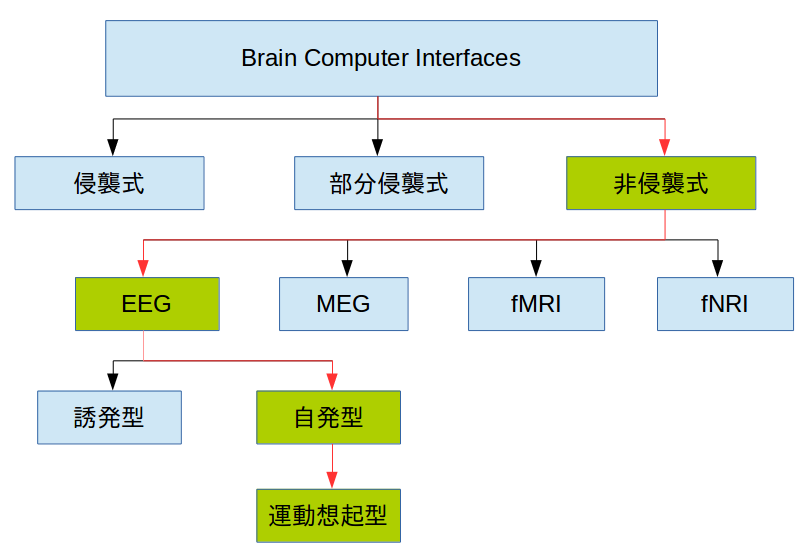
\includegraphics[width=14cm]{images/BCIclass.png}
    \caption{BCIの分類と本研究の焦点}
    \label{fig:BCIclass}
\end{figure}

\subsubsection{\rm BCI\mc の動作原理}
BCIの動作は以下のスキームに従う。
\begin{enumerate}
    \item 脳信号の獲得:センサによりアナログ信号を獲得しディジタル信号へ変換
    \item 信号の前処理:データの成形及びアーチファクトの除去
    \item 特徴量抽出:神経科学や統計に基づいた特徴量の選定
    \item 分類:特徴量から閾値に基づいて意図を分類
    \item 制御信号出力:分類結果に基づいて外部機器へ信号を出力
\end{enumerate}
BCIの種類に関わらず動作原理の根本は同様であるが、
スキームのどの段階に課題が生じるかは異なる。
侵襲式の場合は脳信号の獲得自体が非常に困難であり、安全性やメンテナンス性に課題が生ずる。
非侵襲式の場合は脳信号の獲得は気軽に実施できるが、空間分解能や時間分解能の問題、あるいは
アーチファクトに存在によって意図を復元することは容易ではない。

EEGの場合は個々の脳細胞の活動時に発生した電位の総和を頭皮上で測定しており、深さの情報は失われている。
これは侵襲式計測やMEGおよびfMRIに対する明確な欠点である。
また、頭蓋骨や人体の細胞を電位がどのように伝搬しているかは定かではないため、頭皮上の位置と
脳の表面のみを考えた場合でも位置情報は不明瞭となる。これは部分侵襲式に対する欠点となる。
従ってEEGを用いた運動想起型BCIに焦点を当てる場合、主に特徴量抽出と分類の段階が課題となる(図\ref{fig:BCIsystem})。

\begin{figure}[tb]
    \centering
    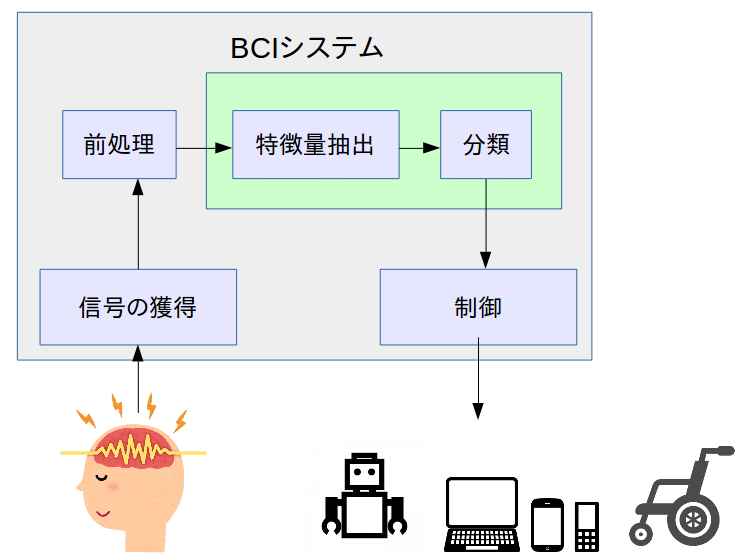
\includegraphics[width=14cm]{images/BCIsystem.png}
    \caption{BCIのスキームと課題点}
    \label{fig:BCIsystem}
\end{figure}

\subsubsection{\mc 運動想起型\rm BCI\mc 周辺の研究}
運動想起時には運動野付近で特定の周波数帯域において活動電位が減少する
事象関連脱同期(Event Related Desynchronization : ERD)の存在が知られており、
神経科学的な、あるいはBCI応用のための研究が盛んに行われている\cite{ERDとERS,ERDリハビリ,運動フィードバック}。
従って特徴量としてERDが用いられる研究も数多くあり、EEGを用いた運動想起型BCIでも基礎となっている\cite{プリミティブERD,Beta波によるBCI,waveletFSVM}。
ERDを発見することができた場合、EEGの振幅あるいはパワーに閾値を設けて分類を行うことができる。
具体的にはスペクトル解析によって各周波数のパワーを推定し、パワーに閾値を設けることとなる。
しかし、EEGからのERDの検知は必ずしも容易ではない。
ERDが生じる頭皮上の位置と周波数は個人差がある上、
有効な周波数スペクトル解析に関しても未だ研究段階である\cite{時間周波数解析の比較}。

また、人の随意運動の約0.5秒から1秒前に現れる運動準備電位も特徴量になると考えられている。
実動作以前に発生するという極めて特殊な現象であるため、
その特性からBCIが人の意志に対して優れた反応速度で動作することが期待される。
BCIの研究としては実肢体動作の分類\cite{運動準備電位肢体}や実指動作の分類\cite{運動準備電位指}などがある。
実運動を行わなくとも運動準備電位が特徴量として活用できるという研究\cite{運動準備電位想起,運動準備電位想起2}もある。

一方で特定のEEGの現象を直接獲得せずに運動想起型BCIを構築する手法も提案されており、
それらの多くが統計的信号処理や機械学習を活用したものである。
特にCommon Spatial Pattern(CSP)と呼ばれる統計的信号処理\cite{CSP1990,CSP1999}は、
EEG解析のために発案されて以降、現在までに様々な派生手法を生み出している\cite{csssp,正則化CSP,カーネルCSP,cvscsp}。
その中でもFilter Bank Common Spartial Pattern\cite{fbcsp}と呼ばれるCSPの
発展手法は、ERDに基づくBCIも含め他の手法と比べ高い性能を有している。

現在、EEGの現象として知られている既知の特徴量を検知する手法から、
機械学習や統計的信号処理を活用した特徴量抽出手法と高度な分類器を組み合わせ
高い性能を発揮する手法の模索が行われている\cite{BCIの比較}。
